\documentclass{article}
\usepackage{graphicx}
\usepackage[margin=1in]{geometry}
\usepackage{caption}
\usepackage{multirow}
\usepackage{array}
\usepackage{hyperref}
\usepackage{listings}
\usepackage{hyperref}
\graphicspath{ {./images} }
\title{Design Document}
\author{
	Politecnico di Milano\\
	Merlino Lorenzo \& Iodice Andrea
}

\date{\today}
\begin{document}
\maketitle
\tableofcontents
\newpage
\section{Introduction}
\subsection{Purpose}
The System to Be will allow users to take part in coding battles. Each coding battle will be part of a tournament and consists of a coding project to be completed.
Educators will create tournaments and create battles by supplying the project structure. 
Students will be able to create teams and the teams will be able to submit a solution to the coding battle. Each solution will be scored using different criterias, such as the amount of test cases passed, amount of time required to submit the solution and quality of the code provided.
Some criteria will be automatically asserted and the remaining ones will be asserted by the creator of the battle.
\subsection{Scope}
CodeKataBattle (CKB) is a new platform that helps students improve their software development skills by training with peers on code kata. 
\\\\
Educators use the platform to challenge students by creating code kata battles in which teams of students can compete against each other, thus proving and improving their skills. 
\\\\
Educators create tournaments to which students can enroll. After enrolling in a tournament students can take part in code kata battle by joining or creating a team.
\\\\
A code kata battle is a programming exercise.
The exercise includes a brief textual description and a software project with build automation scripts that contains a set of test cases that the program must pass.
\\\\
Teams participating in a battle are expected to follow a test-first approach and develop a solution that passes the required tests. Groups deliver their solution to the platform before the deadline.
At the end of the battle, the platform and the educators assign scores to groups, in order to create a competition rank.
\\\\
A Educator cannot be a student and vice versa.
\subsection{Definitions, Acronyms, Abbreviations}
\subsubsection{Definitions}
\begin{itemize}
\item \textbf{Coding Battle}: programming exercise proposed by an Educator in the context of a tournament.
\item \textbf{Tournament}: a series of coding battles, in which Students can take part as teams. It’s created and managed by an Educator.
\item \textbf{Team}: group of students who enroll in a tournament. Students in the same team work together and the solution they submit will be taken into consideration for each member of the team.
\item \textbf{Rank}: position of a Student in a tournament’s leaderboard, which is calculated on each Student’s score.
\item \textbf{Score}: points gained by a Student by submitting a solution to a Coding Battle.
\item \textbf{Open battle}: a battle that accepts new submissions.
\item \textbf{Closed battle}: a battle that doesn’t accept new submissions but some still need to be evaluated.
\item \textbf{Completed battle}: a battle that doesn’t accept new submissions and where all the submissions have been evaluated.
\item \textbf{Open tournament}: A tournament where new battles can be created.
\item \textbf{Closed tournament}: A tournament where new battles cannot be created but some are still not completed.
\item \textbf{Completed tournament}: A tournament where new battles cannot be created and all battle have been completed
\item \textbf{Team leader}: Student who created the team.
\item \textbf{Automated grading}: A series of scores that is automatically assigned to a solution, it is composed of:
\begin{itemize}
\item Number of test passed
\item Time passed after the battle publication
\item Static analysis result
\end{itemize}
\item \textbf{User}: either a Student or an Educator
\item \textbf{Educator}: user of the system, who manages tournaments and battles.
\item \textbf{Student}: user of the system, who participates in tournaments and battles.
\end{itemize}
\subsubsection{Acronyms}
\begin{itemize}
\item \textbf{RASD}: Requirements Analysis and Specification Document
\item \textbf{DD}: Design Document
\end{itemize}
\subsubsection{Abbreviations}
\begin{itemize}
\item \textbf{[Rn]}: the n-th requirement
\item \textbf{[UCn]}: the n-th use case
\end{itemize}
\subsection{Revision History}
\begin{itemize}
\item Version 1.0
\end{itemize}
\subsection{Reference Documents}
\begin{itemize}
\item The specification of the RASD and DD assignment of the Software
Engineering II course, held by professor Matteo Rossi, Elisabetta Di Nitto and
Matteo Camilli at the Politecnico di Milano, A.Y 2023/2024;
\item Slides of Software Engineering 2 course on WeBeep;
\item DD Sample from A.Y. 2022-2023
\item \href{https://docs.github.com/en/rest?apiVersion=2022-11-28}{Github API documentation}
\end{itemize}
\subsection{Document Structure}
Mainly the current document is divided in 7 chapters, which are:\\
\begin{enumerate}
\item Introduction: The first chapter includes the introduction in which is explained
the purpose of the document, then, a brief recall of the concepts introduced in
the RASD is given. Finally, important information for the reader is given, i.e.
definitions, acronyms, synonyms and the set of documents referenced.
\item Architectural Design: it includes a detailed description of the architecture of
the system, including the high level view of the elements, the software
components of CKB, a description through runtime diagrams of various
functionalities of the system and, finally, an in-depth explanation of the
architectural pattern used.
\item User Interface Design: are provided the mockups of the application user
interfaces, with the links between them to help in understanding the flow
between them.
\item Requirements Traceability: it describes the connections between the
requirements defined in the RASD and the components described in the first
chapter. This is used as proof that the design decisions have been taken with
respect to the requirements, and therefore that the designed system can fulfill
the goals.
\item Implementation,Integration and Test Plan: it describes the process of
implementation, integration and testing to which developers have to stick in
order to produce the correct system in a correct way.
\item Effort spent
\item References: it contains the references to any documents and to the Software
used in this document.

\end{enumerate}

\newpage
\section{Architectural design}
\subsection{Overview}
This section describes the overview of the system from a design standpoint, defining its main components and their relationships

\subsubsection{High level view}
The CodeKata system is a distributed system with a four-tier architecture. The four tiers are:
\begin{itemize}
\item Presentation: displays the user interface and manages the user interactions.  
\item Web Server: manages the information sent by the presentation layer, is in charge of load balancing and caching.
\item Application: handles the system logic managing authentication and requests from the presentation layer. It filters access to the data layer
\item Data: maintains all persistent data of the system and the shared data between different instances of the application layer
\end{itemize}

\begin{center}
    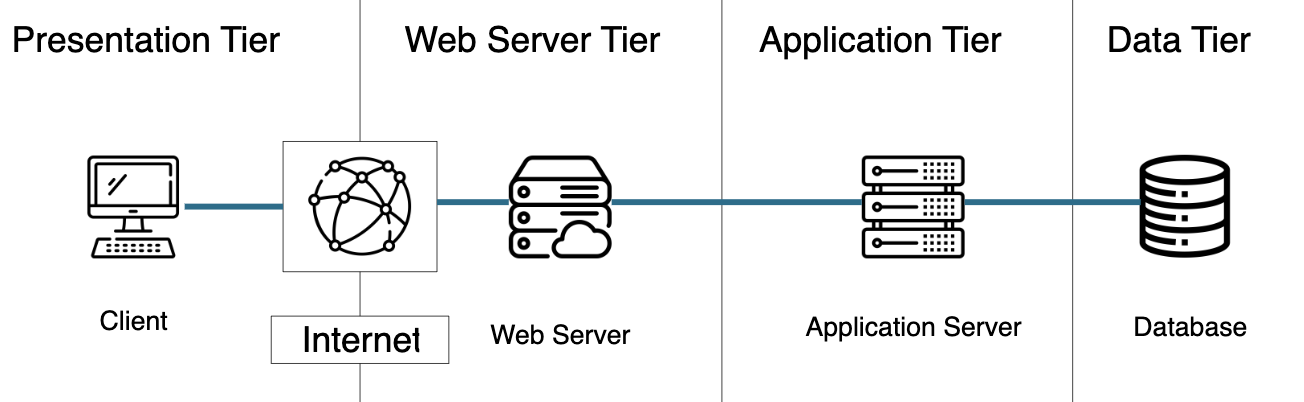
\includegraphics[width=\linewidth]{hlv1.png}
   \captionof{figure}{High level view}
  \label{fig:hlv1}
\end{center}

The communication between client and server through http requests and responses.
The system can be accessed via browser by both Students and Educators. 
\\\\
The presentation tier communicates with the web server layer which is in charge of distributing the request between the multiple application layer instances. 
\\\\
The application tier elaborates the requests and access the data from the data layer. The application tier interfaces with the GitHub api on the user behalf. 
\\\\
User session is identified a by JWT, Json Web Token. it contains the user internal ID, the user Github username and the user Github access token
\begin{center}
    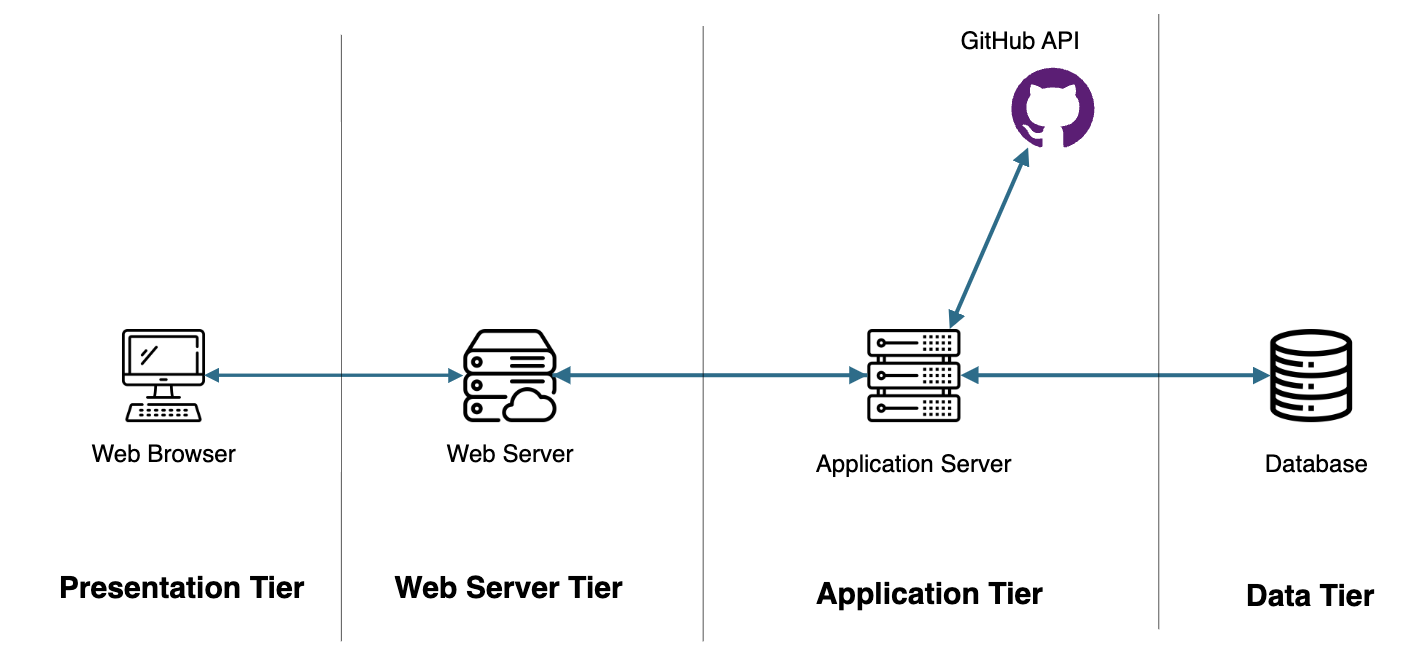
\includegraphics[width=\linewidth]{hlv2.png}
   \captionof{figure}{High level view}
  \label{fig:hlv2}
\end{center}

\subsubsection{Distributed view}
The system has multiple instances of the application tier to meet availability and performance requirements.

\subsection{Component view}
The system is divided into different components, the following diagram describes which components are in the system and how they are connected between each other. 
\\\\
External components that are not part of the system are colored white. Presentation components are colored purple. Web server components are colored green. Application components are colored yellow. Data components are colored blue.
\newpage
\begin{center}
    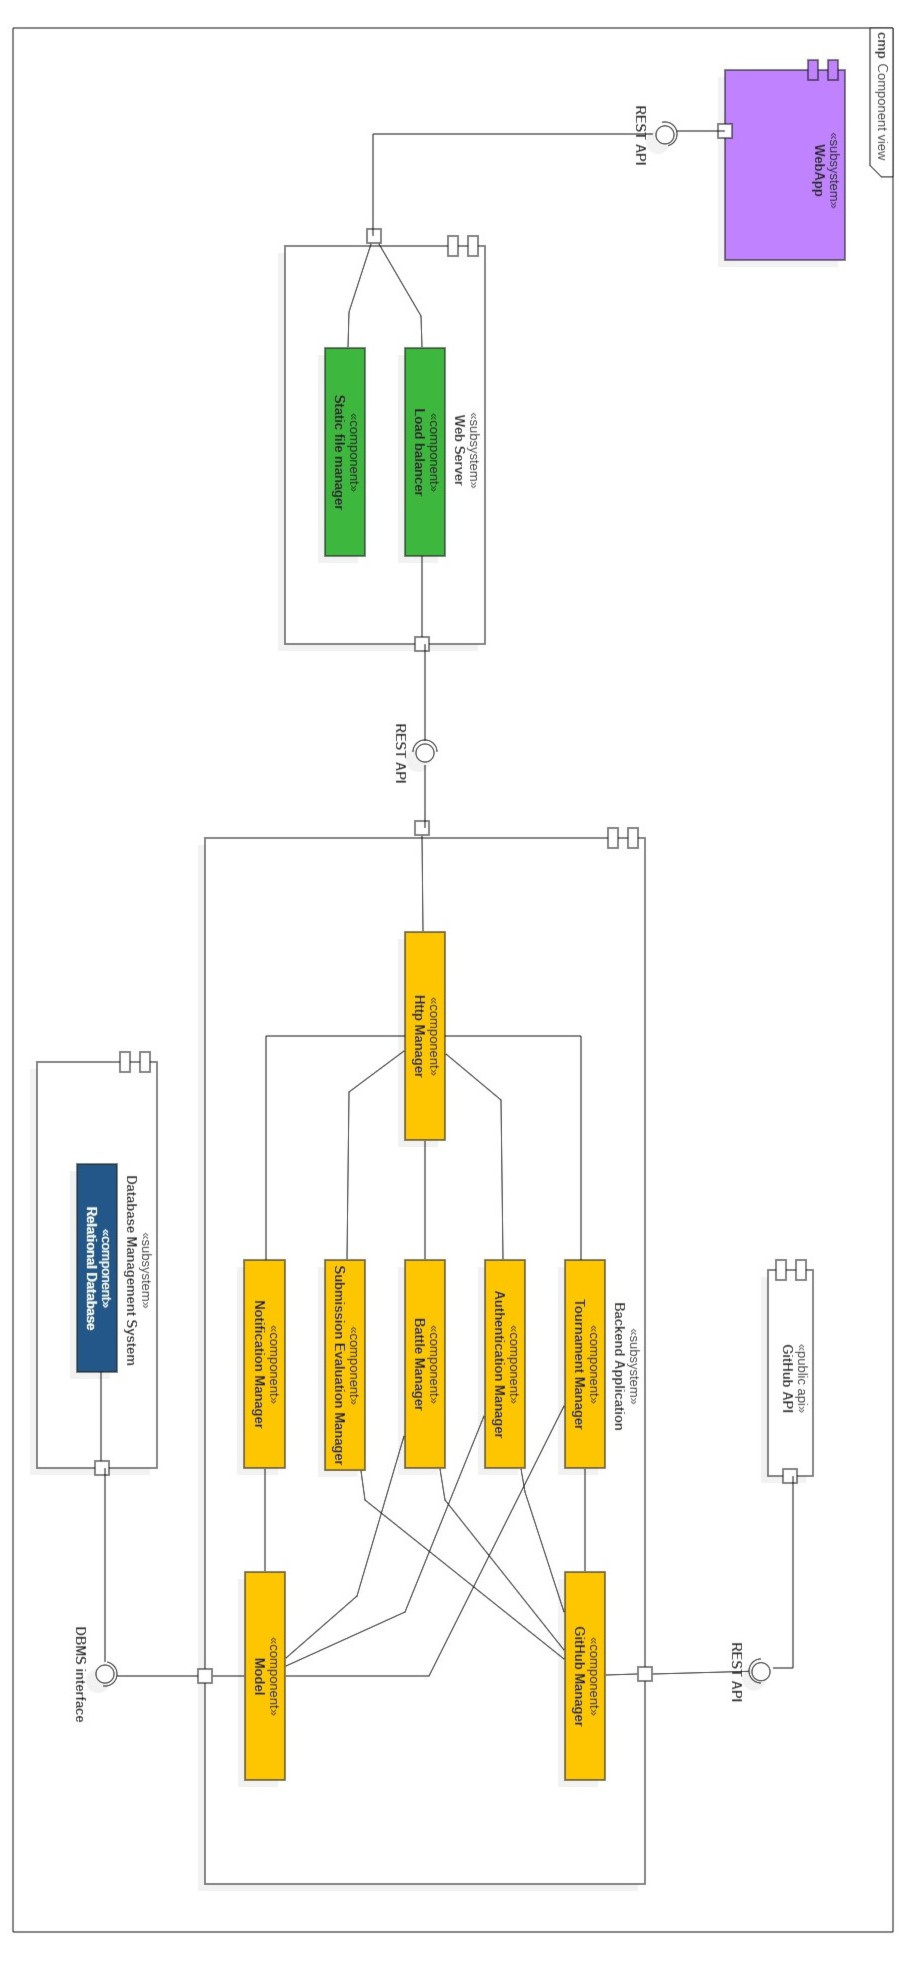
\includegraphics[width=0.6\linewidth]{cv3.jpg}
   \captionof{figure}{Component view}
  \label{fig:cv}
\end{center}
\subsubsection{The Relational Database}
contains all the relevant data to the application and it resolves the queries received from the model component with the requested data.
\subsubsection{The Model}
is used to store the data that are part of the persistent state of the system (which in our case is stored on a database) when this is loaded into the application. Moreover, it provides all the methods that are necessary to access those data and it also implements the logic to manipulate them. In other words: whenever some data contained in the database is needed by any component of the system, for any kind of computation, they delegate the task of retrieving such information to the model component. It not only retrieves them but it also stores them in ad-hoc data structures so that they are ready to be used for the required computations. The model component is the only one interacting with the Relational Database. 
\subsubsection{The GitHub Manager}
manages all interactions between components and the GitHub api.
\subsubsection{The Notification Manager}
registers the notification’s creation and manages its internal status until deletion. It interfaces with the model to record new notifications, retrieve existing ones and delete old ones
\subsubsection{The Authentication Manager}
handles the user login and interfaces with the GitHub Manager to verify the user access token. It interfaces with the model to record the access token or retrieve user info.
\subsubsection{The HTTP Manager}
handles http requests and manages the http sessions. 
\subsubsection{The Battle Manager}
handles battles’ creation and updates their status when needed. When creating a battle it verifies that the battle configuration is valid, handles teams creations, teams joins and team invites. It interfaces with the Notification manager to notify invites to join a team, when a Student joins a team and when a battle is created or closed. Interfaces with the database to record battles and teams data.
\subsubsection{The Tournament Manager}
handles the creation of tournaments, the additions of allowed educators into the tournaments, the enrollment of students into tournaments and the status of the tournaments. It interfaces with the database to record and retrieve tournament data.
\subsubsection{The Submission Evaluation Manager}
handles the automatic grading of new submissions of open battles. Handles manual grading of closed battles. Interfaces with the database to record the team gradings. 
\subsubsection{The Web-App}
is the web interface used by users to access the system and interact with it. It sends requests to the Web Server via HTTP and shows the user the responses from the system.
\subsubsection{The Web Server}
manages incoming requests from the Web-App component and distributes them between the application’s instances. Handles the distributions of static files to the Web-App.

\subsection{Deployment view}
\begin{center}
    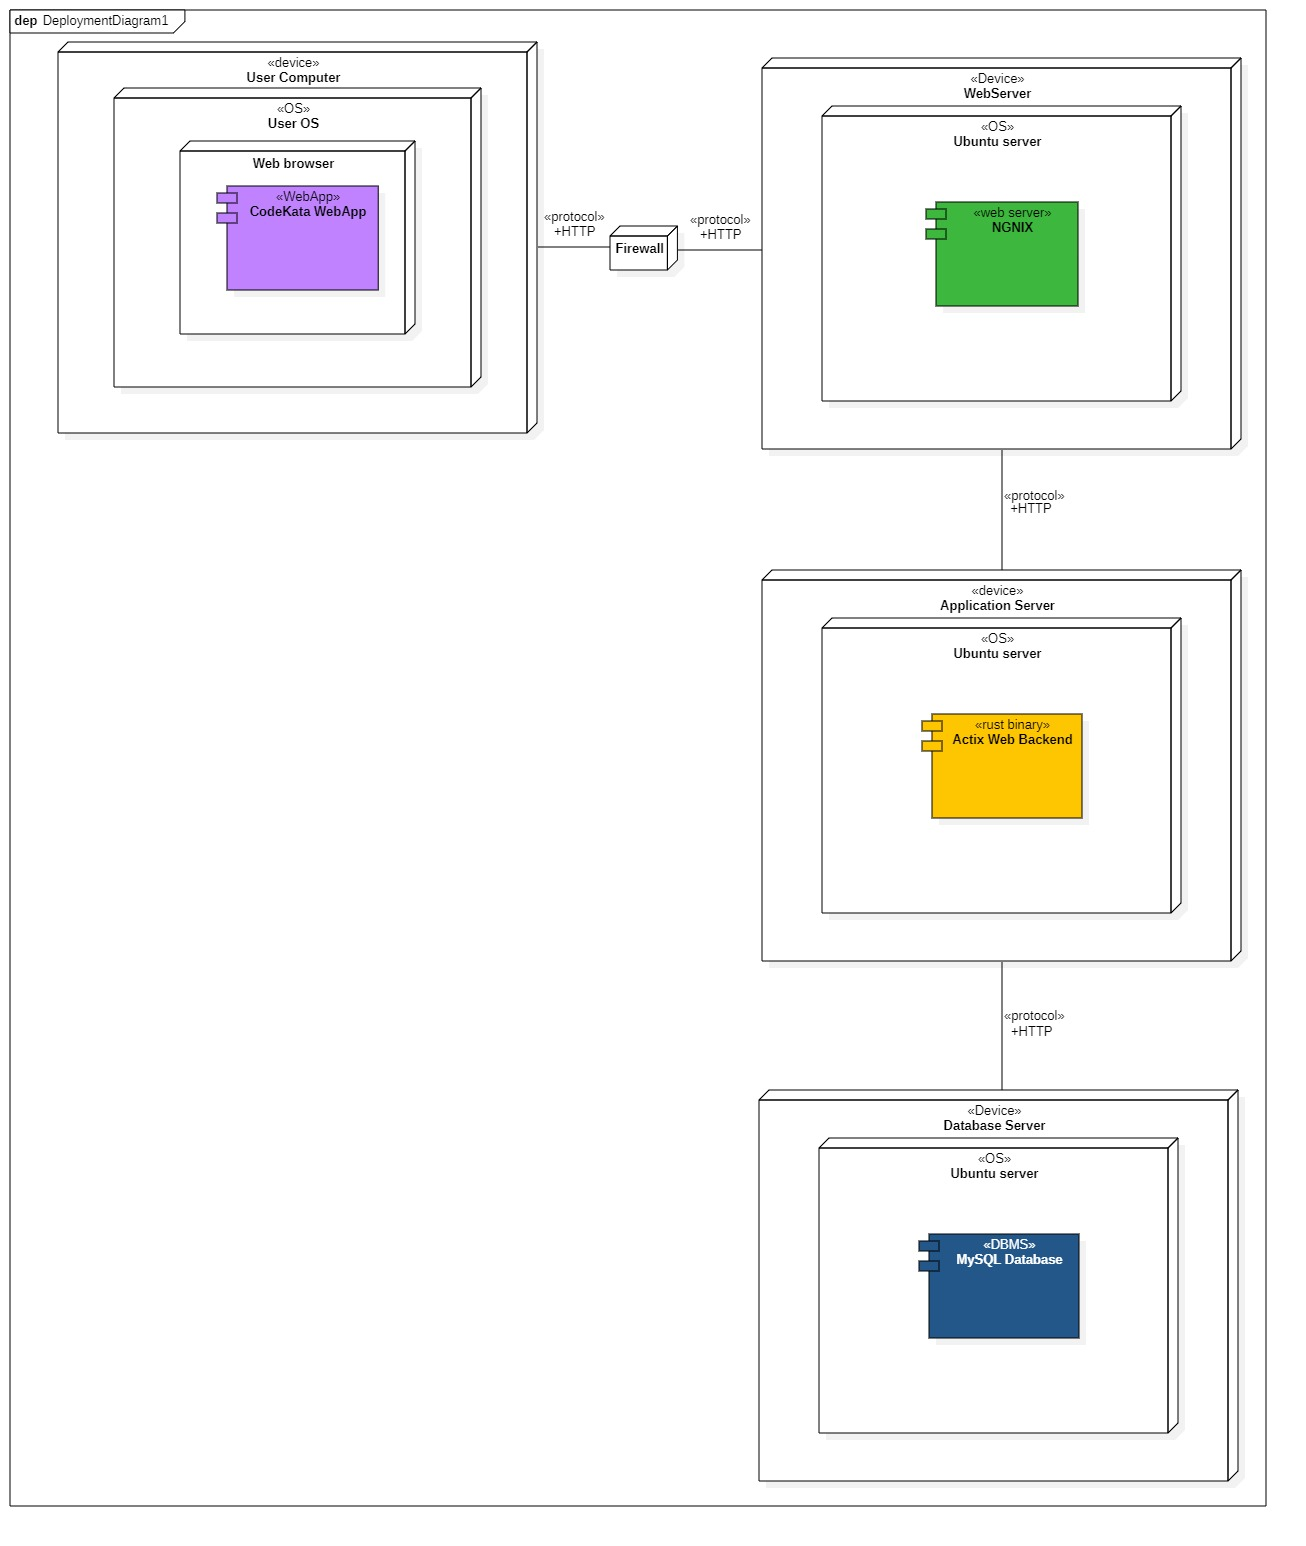
\includegraphics[width=0.9\linewidth]{dv.jpg}
   \captionof{figure}{Deployment view}
  \label{fig:dv}
\end{center}
Further details about the elements in the graph are provided in the following.
\begin{itemize}
\item \textbf{Firewall} is a device that monitors the packets incoming to the system, if a packet is potentially dangerous it is not forwarder. It is placed before the Web Server and allows incoming packers only if directed to the web server with the correct port and the correct protocol, in this way the only packets that enter the network are considered safe.
\item \textbf{Computer} is a regular computer used by the user. No special applications are required to be installed on it, except for a web browser. This will be necessary to surf the internet and reach the CKB web page. An HTTPS connection with the system is established by passing through a firewall and after the forwarding, operated by the designated load balancer, to an available application server. 
\item \textbf{Web server} receives all the requests sent from the web app. It then forwards the received request to the different instances of the application allowing for the incoming load to be balanced on the different instances . It also distributes the web app static files and handles the caching of requests when needed.
\item \textbf{Application server} receives all the requests sent from the web server and elaborates them. It sends requests to the Database server to read and write data when needed. It communicates directly with the GitHub api.
\item \textbf{Database server} host the relational database that contains all the system data it is accessed by the application server.
\end{itemize}

\newpage
\subsection{Runtime views}
\begin{center}
    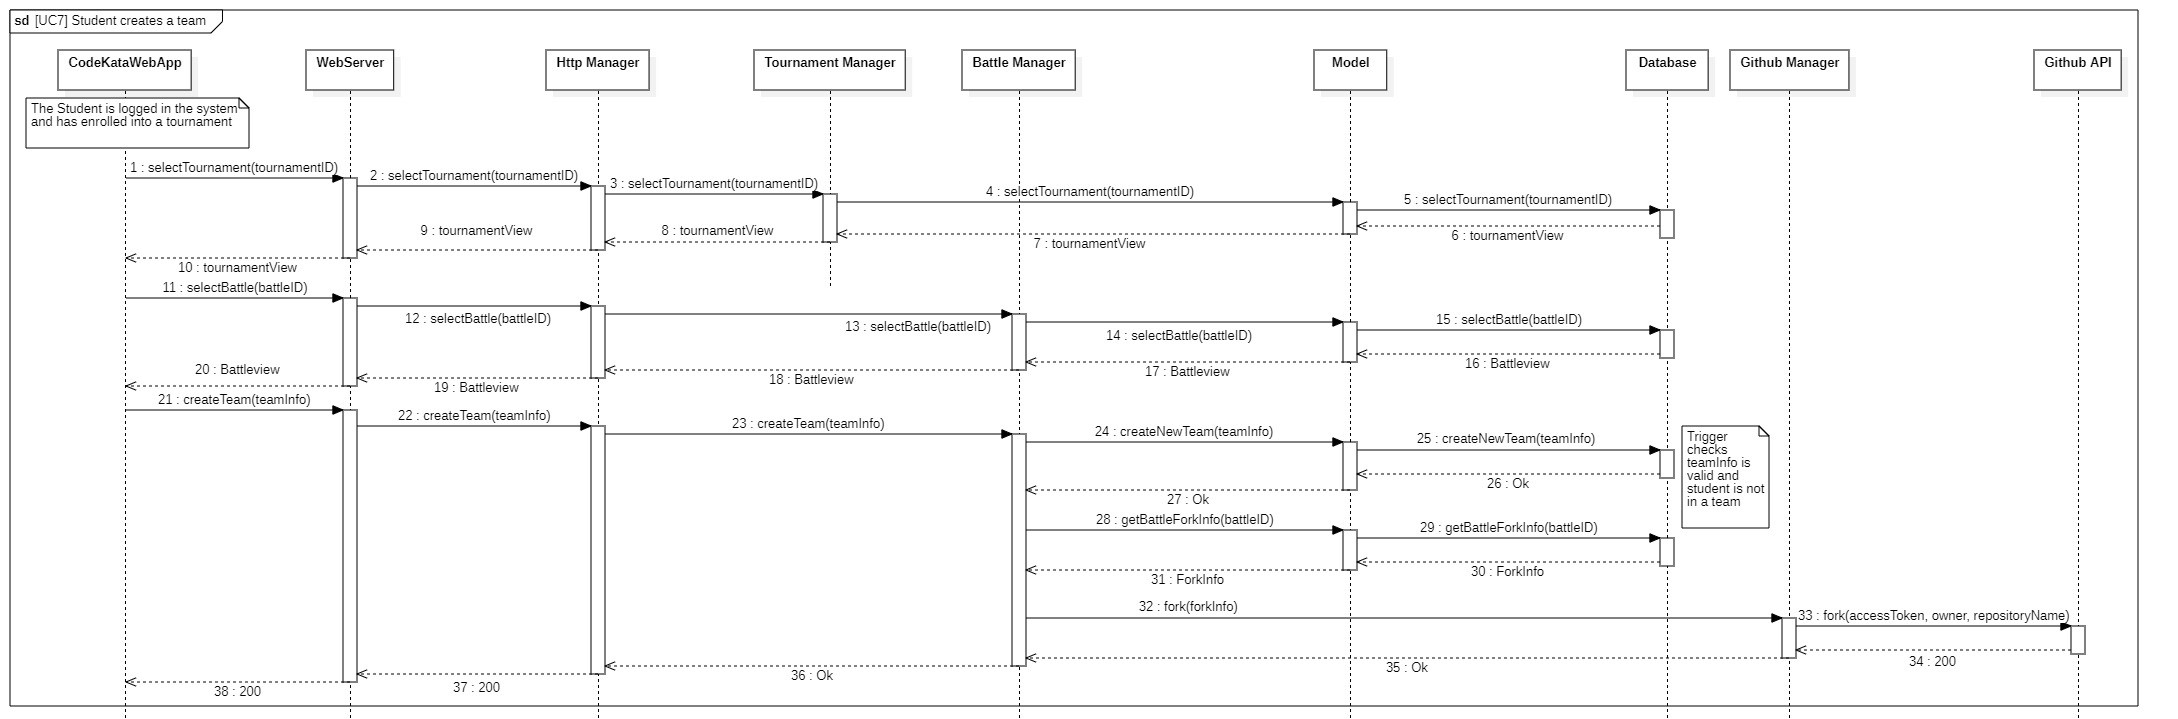
\includegraphics[angle=90,width=0.4\linewidth]{uc7.jpg}
   \captionof{figure}{UC7}
  \label{fig:uc7}
\end{center}

\newpage
\begin{center}
    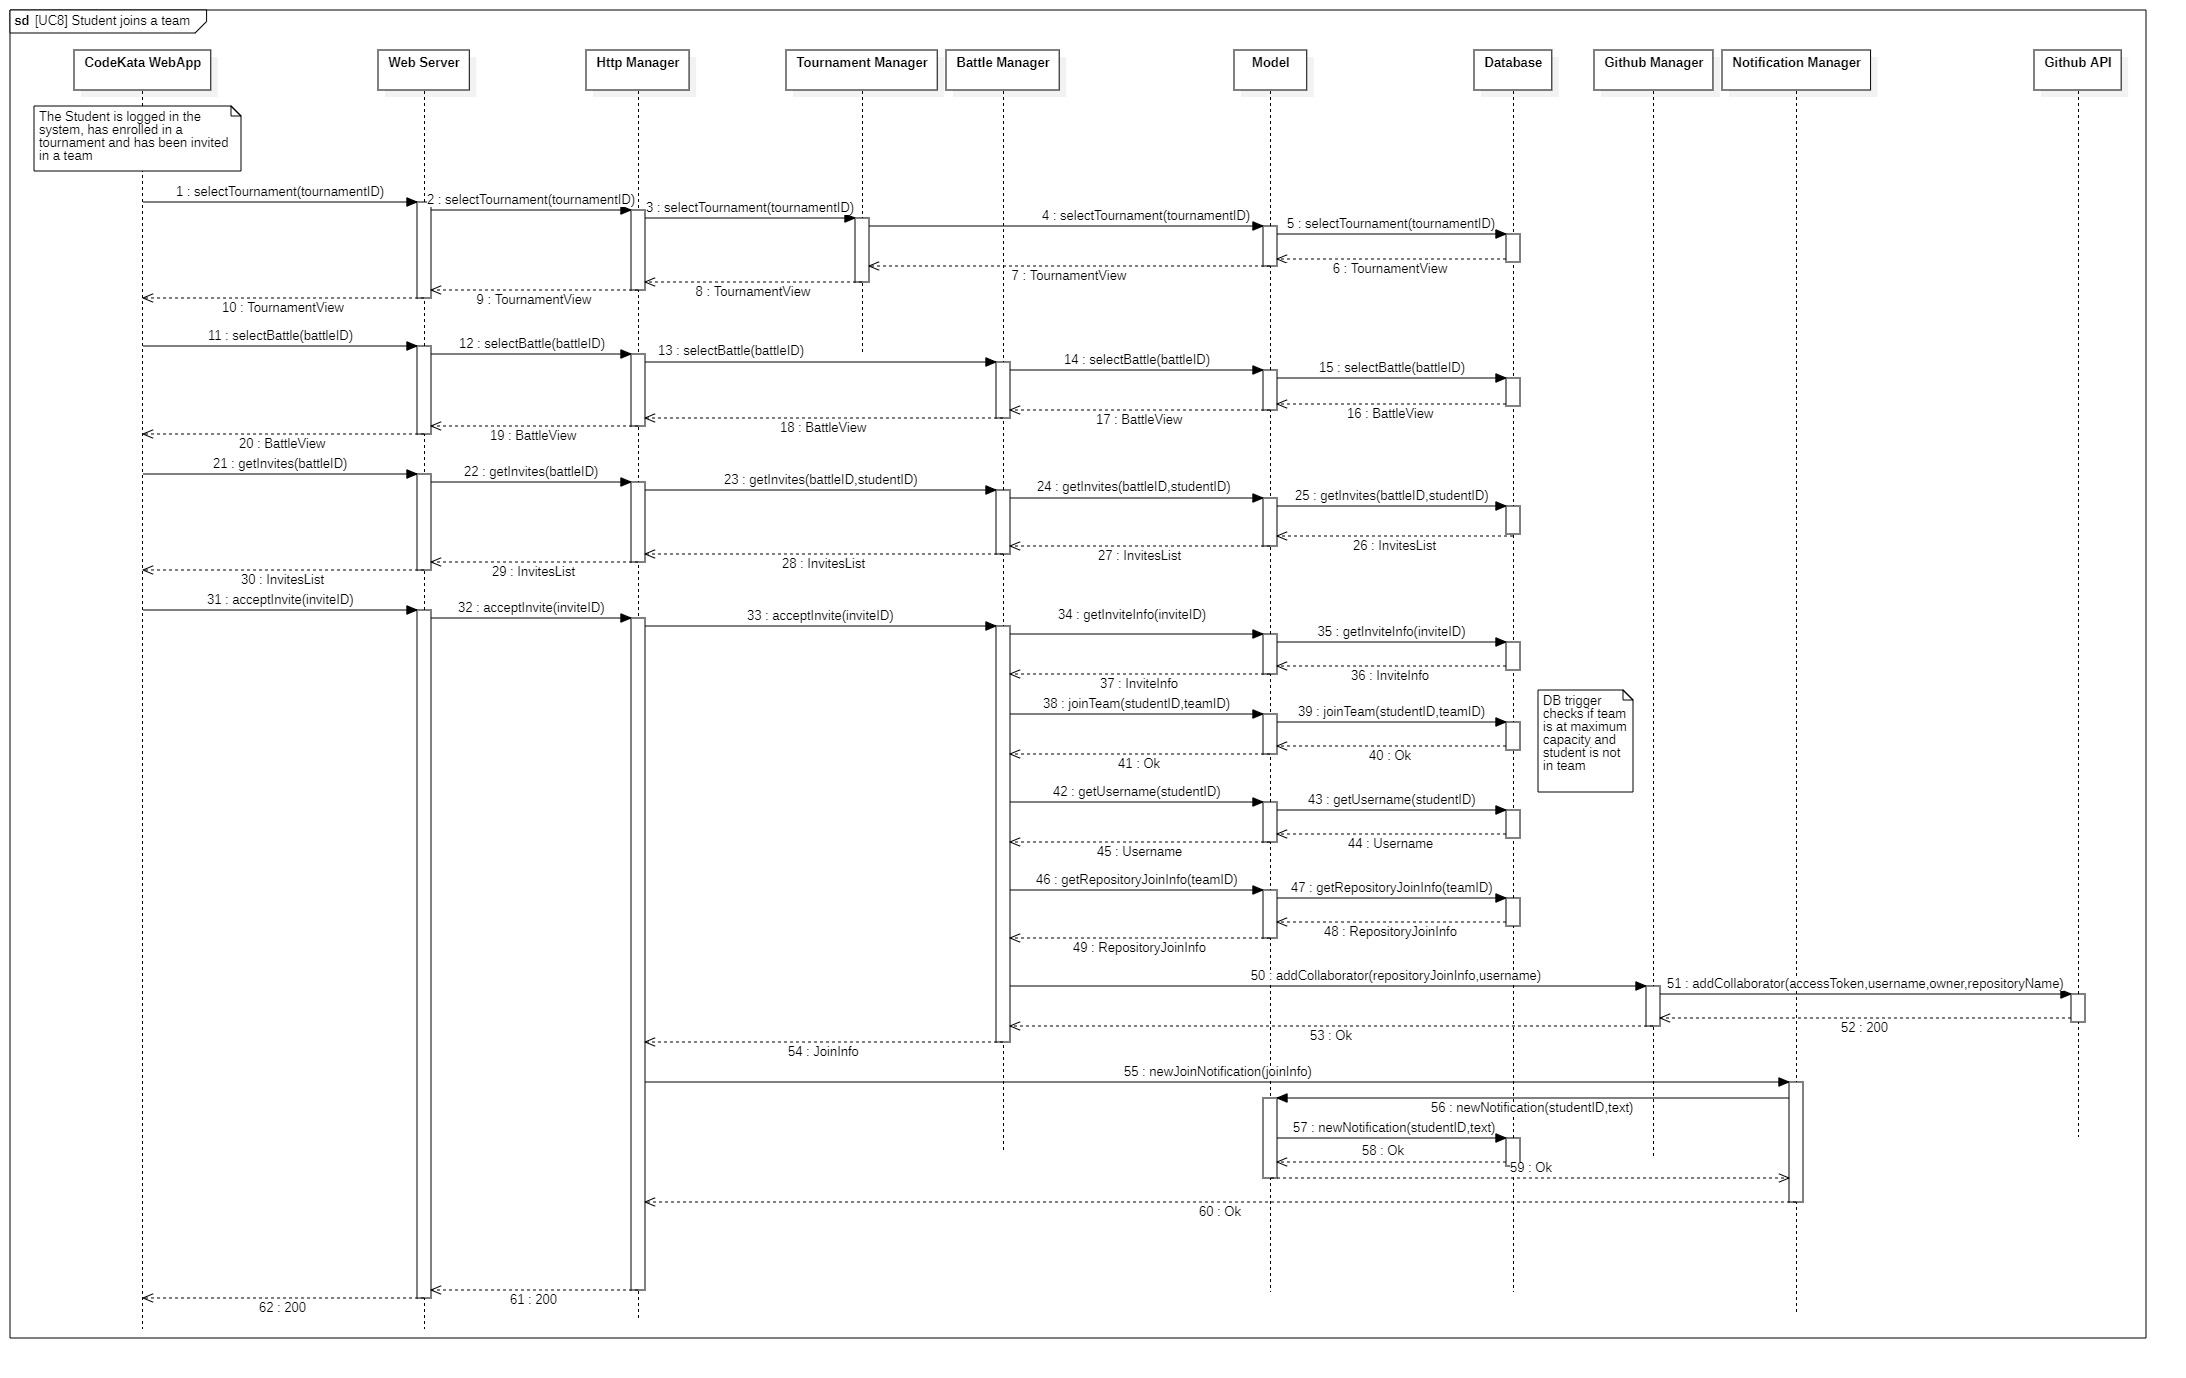
\includegraphics[angle=90,width=0.8\linewidth]{uc8.jpg}
   \captionof{figure}{UC8}
  \label{fig:uc8}
\end{center}

\newpage
\begin{center}
    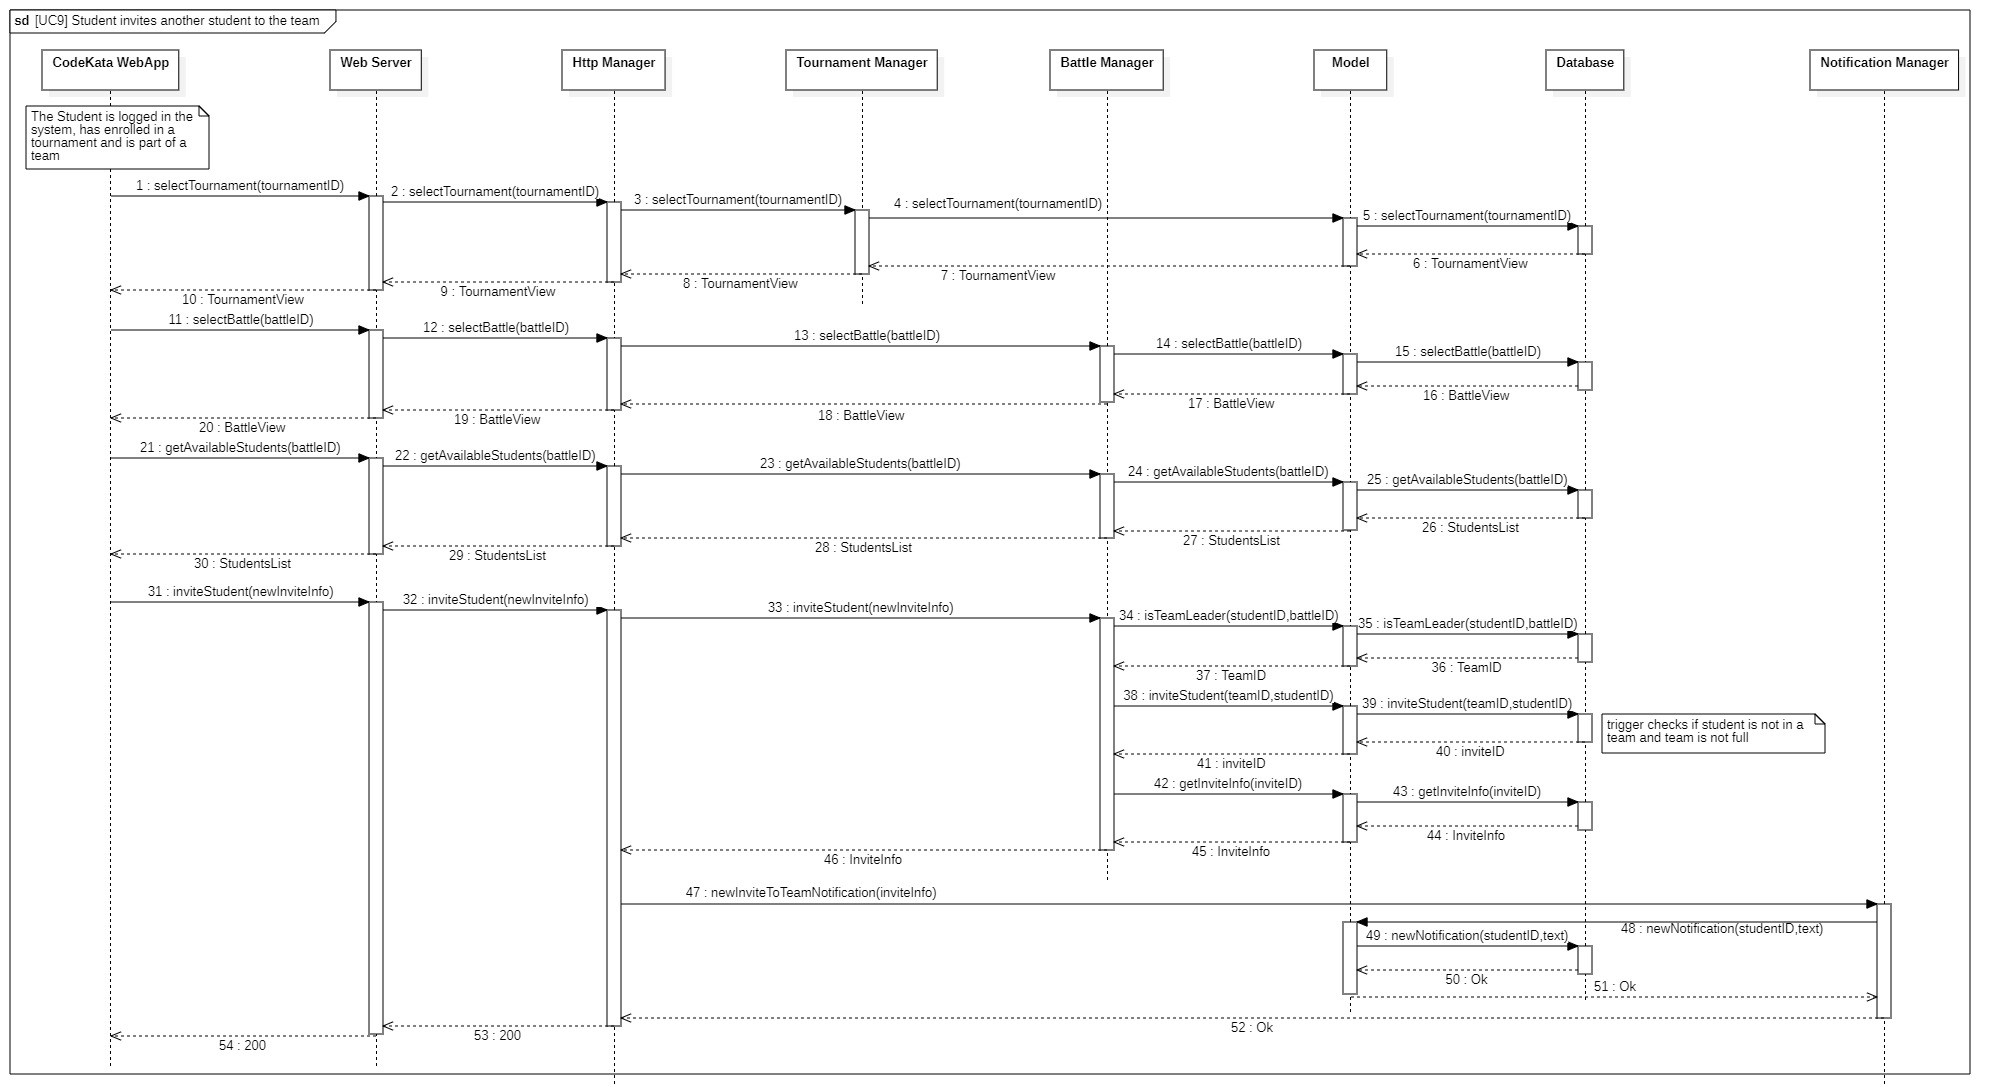
\includegraphics[angle=90,width=0.7\linewidth]{uc9.jpg}
   \captionof{figure}{UC9}
  \label{fig:uc9}
\end{center}

\newpage
\begin{center}
    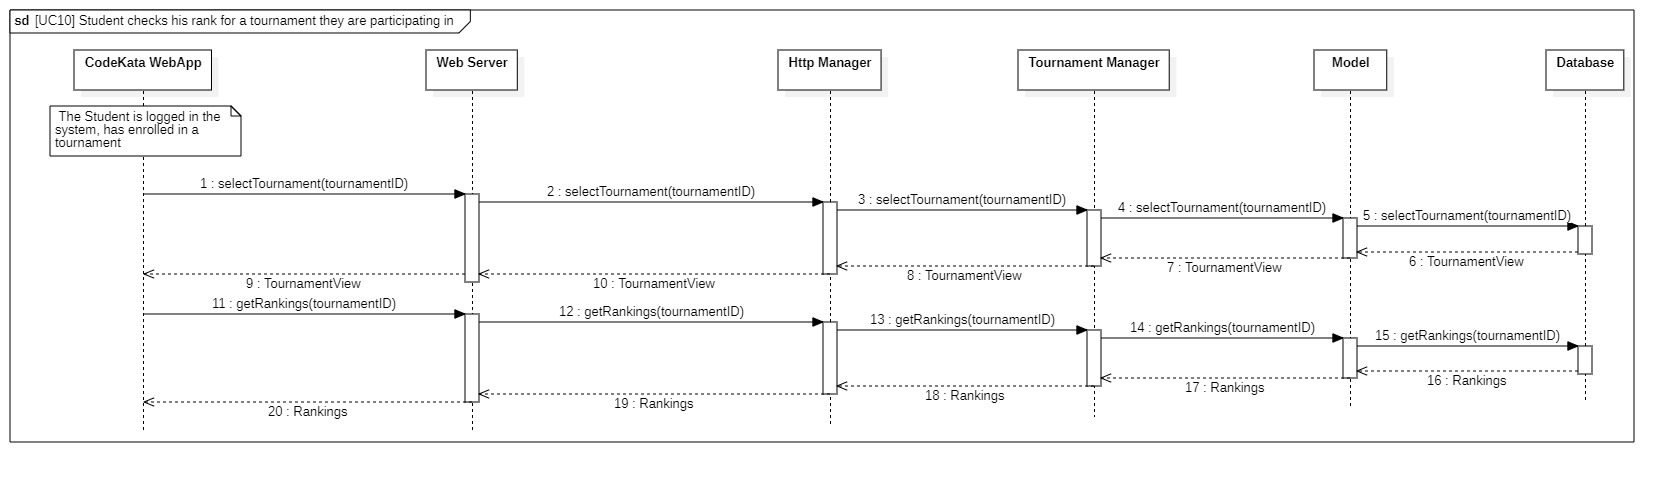
\includegraphics[angle=90,width=0.37\linewidth]{uc10.jpg}
   \captionof{figure}{UC10}
  \label{fig:uc10}
\end{center}

\newpage
\begin{center}
    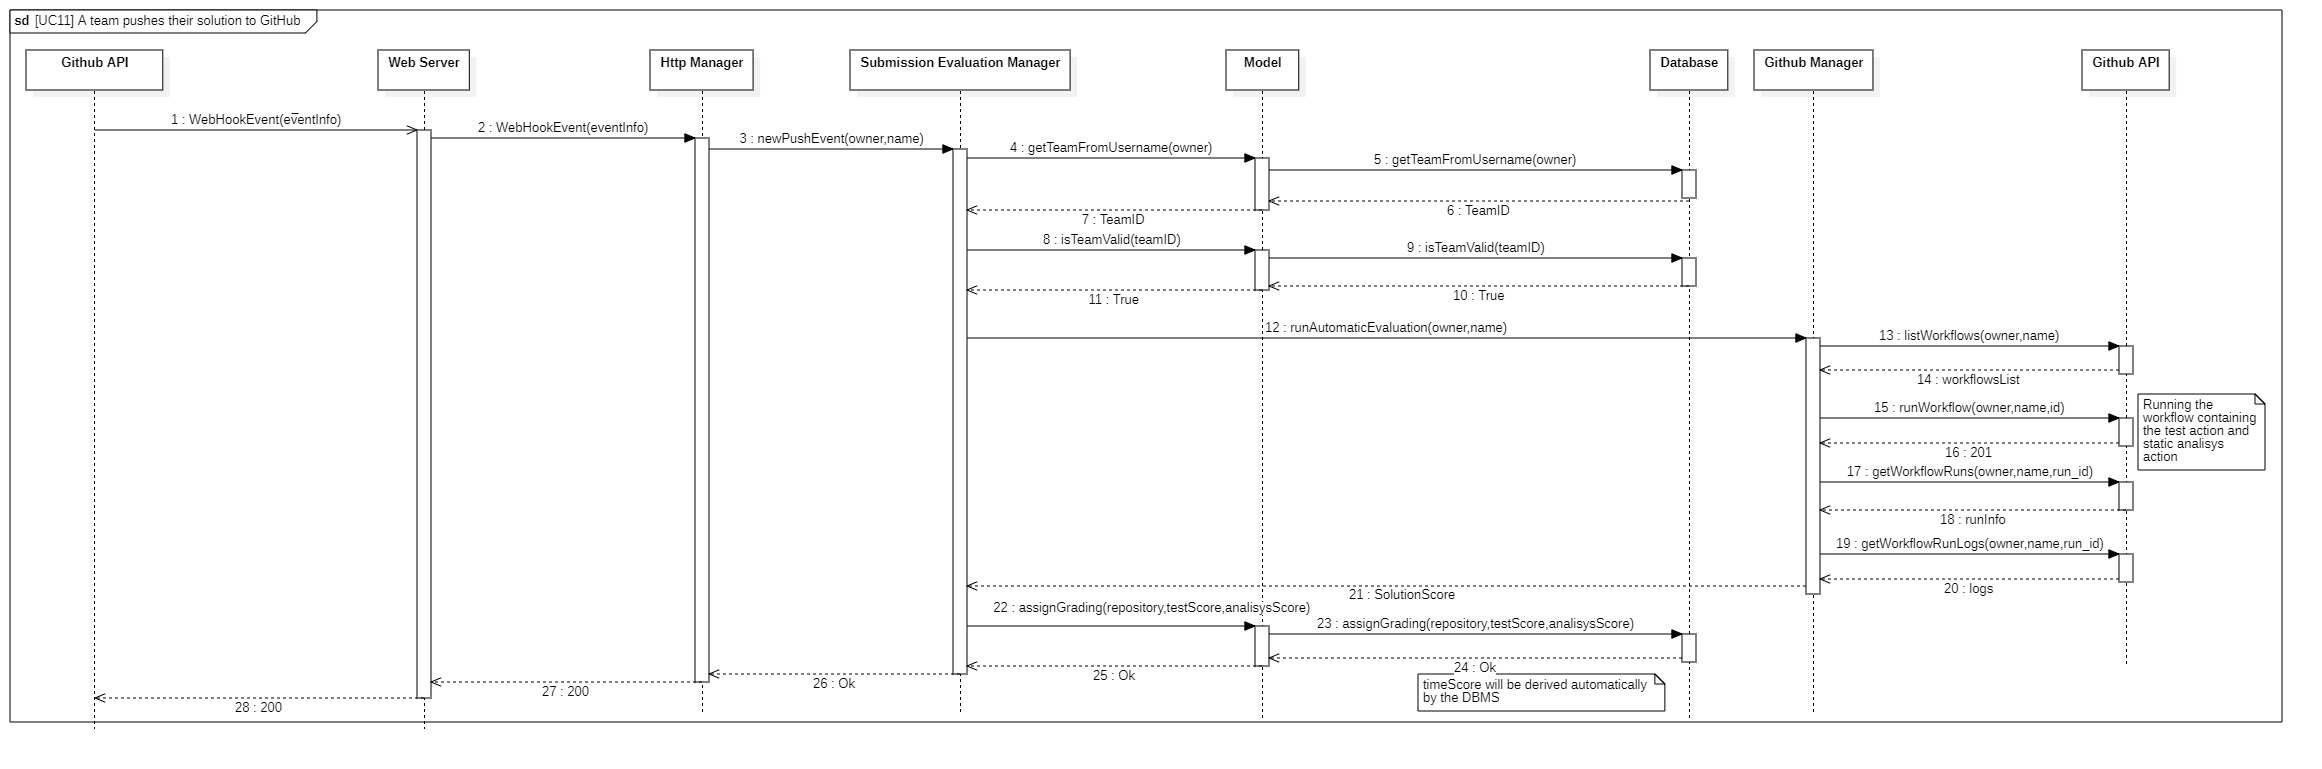
\includegraphics[angle=90,width=0.4\linewidth]{uc11.jpg}
   \captionof{figure}{UC11}
  \label{fig:uc11}
\end{center}

\newpage
\begin{center}
    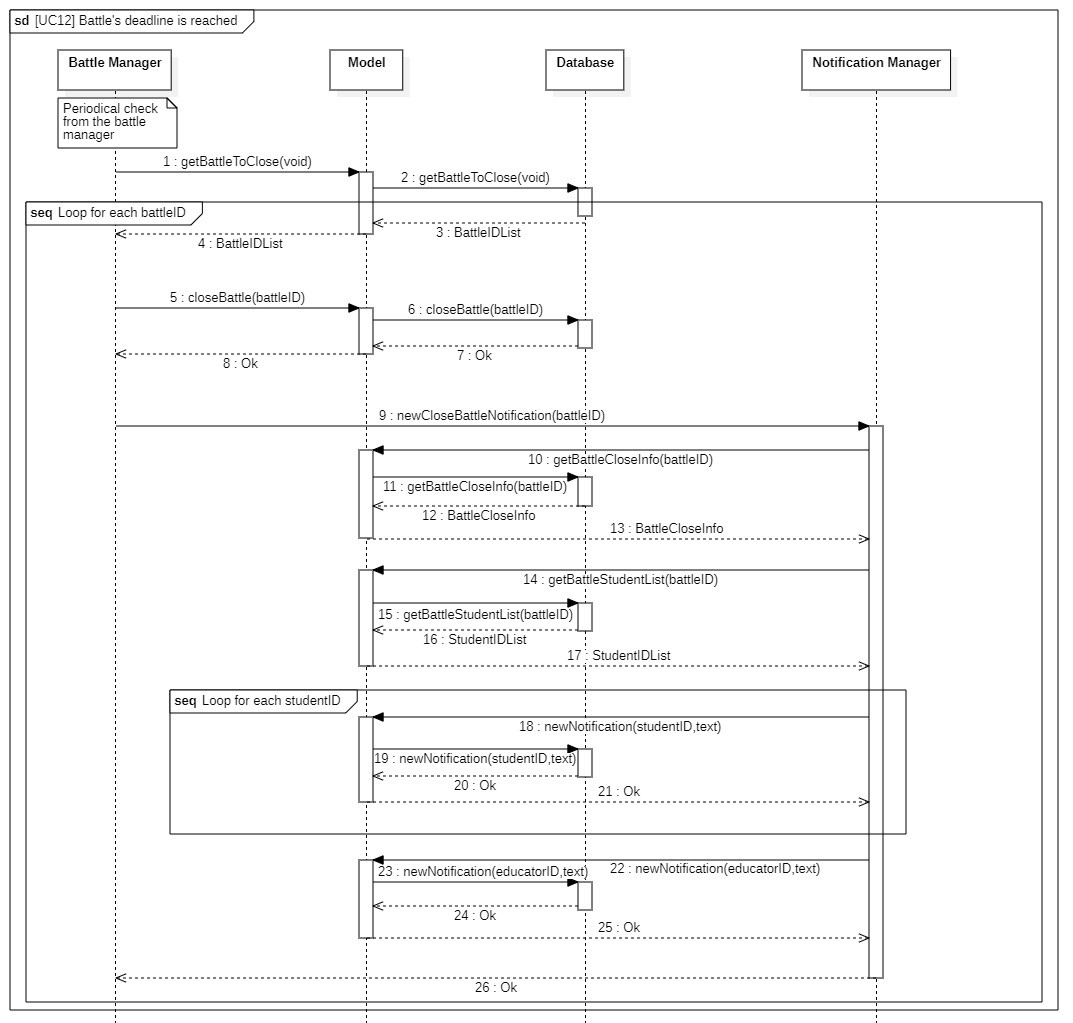
\includegraphics[angle=90,width=\linewidth]{uc12.jpg}
   \captionof{figure}{UC12}
  \label{fig:uc12}
\end{center}

\newpage
\begin{center}
    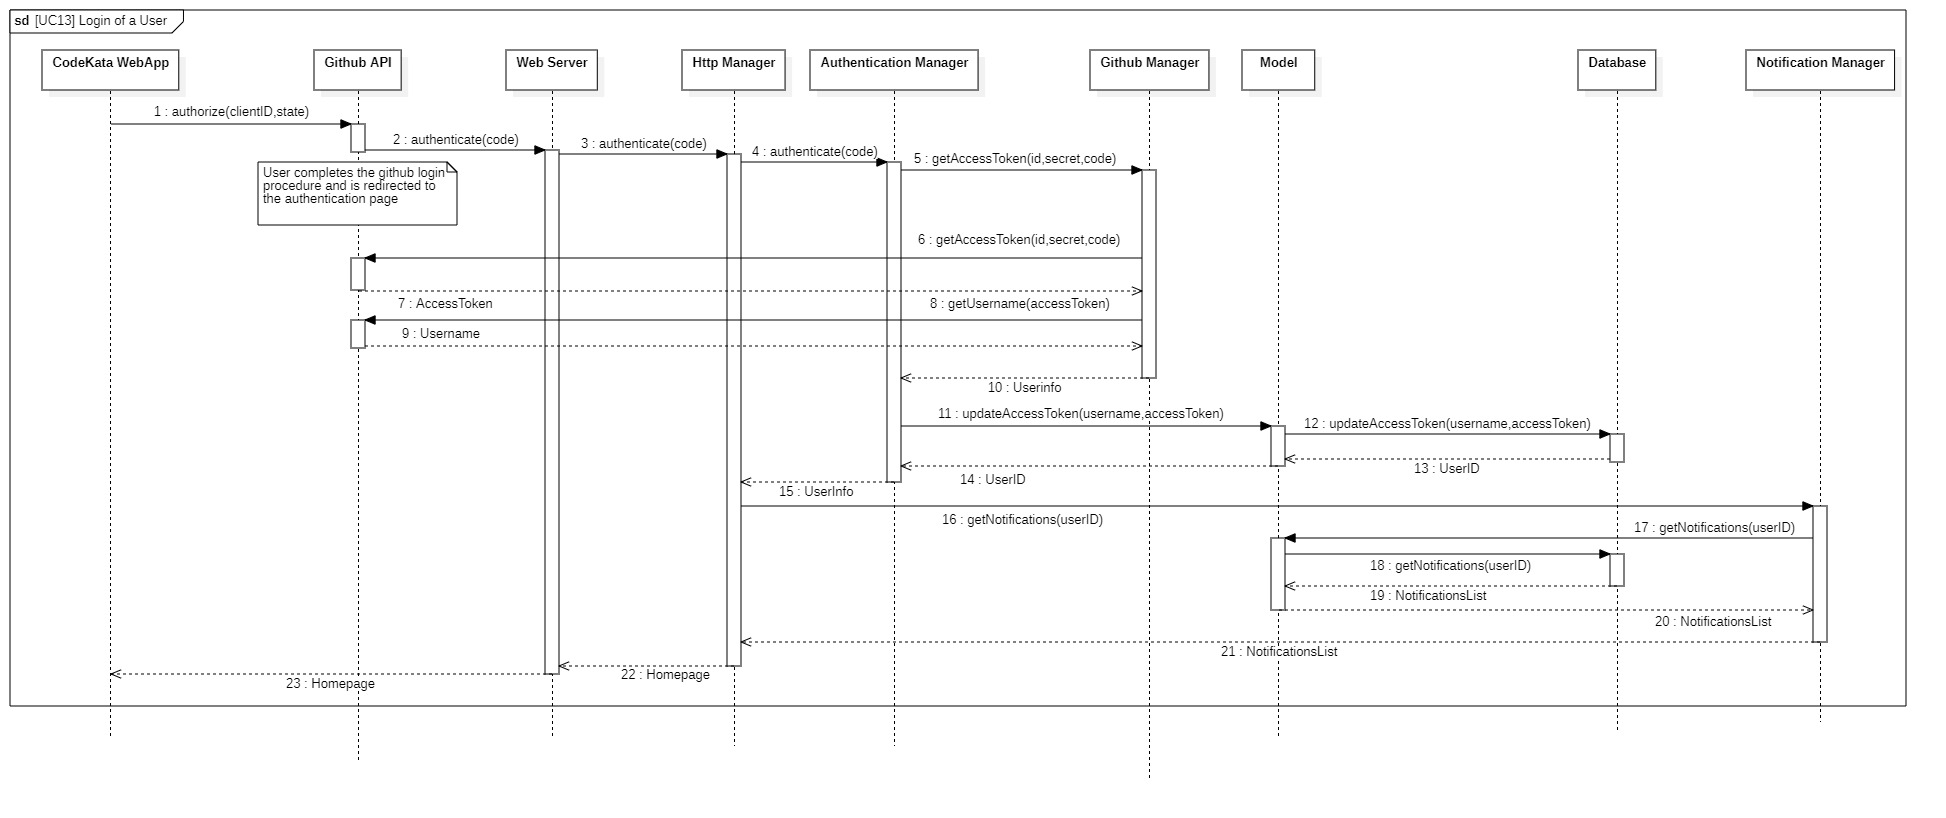
\includegraphics[angle=90,width=0.5\linewidth]{uc13.jpg}
   \captionof{figure}{UC13}
  \label{fig:uc13}
\end{center}

\newpage
\subsection{Component interfaces}
\subsubsection{Web Server}
\textbf{selectTournament(tournamentID)}\\
Rest API call used to get the  tournament view\\
\textit{Param}: tournamentID the ID of the tournament\\
\textit{Returns}: all data needed to build the tournament view if successful\\
\\
\textbf{selectBattle(battleID)}\\
Rest API call used to get the battle\\
\textit{Param}: battleID the ID of the battle\\
\textit{Returns}: all data needed to build the battle view if successful\\
\\
\textbf{createTeam(teamInfo)}\\
Rest API call used create a new team for a battle\\
\textit{Param}: teamInfo the info about the new team\\
\textit{Returns}: 200 if successful\\
\\
\textbf{getInvites(battleID)}\\
Rest API call used to get the invites for the specified battle\\
\textit{Param}: battleID the ID of the battle\\
\textit{Returns}: list of invites and their id if successful\\
\\
\textbf{acceptInvite(inviteID)}\\
Rest API call used to accept an invite to a team\\
\textit{Param}: inviteID the id of the invite\\
\textit{Returns}: 200 if successful\\
\\
\textbf{getAvailableStudents(battleID)}\\
Rest API call used to get the available students for the specified battle\\
\textit{Param}: battleID the ID of the battle\\
\textit{Returns}: list of students usernames and their id if successful\\
\\
\textbf{inviteStudent(newInviteInfo)}\\
Rest API call used to invite a new student\\
\textit{Param}: newInviteInfo info regarding the student being invited and the battle\\
\textit{Returns}: 200 if successful\\

\subsubsection{Http Manager}
\textbf{selectTournament(tournamentID)}\\
Rest API call used to get the  tournament view\\
\textit{Param}: tournamentID the ID of the tournament\\
\textit{Returns}: all data needed to build the tournament view if successful\\
\\
\textbf{selectBattle(battleID)}\\
Rest API call used to get the battle\\
\textit{Param}: battleID the ID of the battle\\
\textit{Returns}: all data needed to build the battle view if successful\\
\\
\textbf{createTeam(teamInfo)}\\
Rest API call used create a new team for a battle\\
\textit{Param}: teamInfo the info about the new team\\
\textit{Returns}: 200 if successful\\
\\
\textbf{getInvites(battleID)}\\
Rest API call used to get the invites for the specified battle\\
\textit{Param}: battleID the ID of the battle\\
\textit{Returns}: list of invites and their id if successful\\
\\
\textbf{acceptInvite(inviteID)}\\
Rest API call used to accept an invite to a team\\
\textit{Param}: inviteID the id of the invite\\
\textit{Returns}: 200 if successful\\
\\
\textbf{getAvailableStudents(battleID)}\\
Rest API call used to get the available students for the specified battle\\
\textit{Param}: battleID the ID of the battle\\
\textit{Returns}: list of students usernames and their id if successful\\
\\
\textbf{inviteStudent(newInviteInfo)}\\
Rest API call used to invite a new student\\
\textit{Param}: newInviteInfo info regarding the student being invited and the battle\\
\textit{Returns}: 200 if successful\\



\subsection{Selected architectural Styles and patterns}
\subsubsection{4-tier Architecture}
CKB will be built over a 4-tier architecture which provides many benefits thanks to the modularization of the system in three independent layers (or tiers):
Presentation tier: Top-level tier including the user’s interface. Its main function is to rearrange the received data from the web and application tiers and present them to the user in a more intuitive and comprehensible manner.
Web Server tier: this tier receives requests via HTTP from the user’s client and redirects them to an application server that is available. After the web server receives the response from the application tier, it will forward the response message to the user. Moreover, this tier is going to have a caching funcion (it will send static files to the user, when required) and a load balancing function: the requests received are sent to a server that has enough resources to elaborate it.
Application tier: It includes the business logic of the application, that is the logic according to which the application takes decisions and performs calculations. Moreover, it passes and processes data between the two surrounding layers.
 Data tier: It includes the Database system and provides an API, to the application tier, for accessing and managing the data stored in the DB
Adopting this type of architecture guarantees a higher flexibility by allowing at first to develop and then to update a specific part of the system apart from the others. Besides, the middle tiers between client and data server ensures a better protection of the stored data. In fact the information is accessed through the application layer instead of being accessed directly by the client.
\subsubsection{Model View Controller pattern}
For implementing the web application, that allows the user to access all the functionalities offered by CKB, was chosen to follow the Model-View-Controller pattern (MVC pattern). It includes three main components:
\begin{itemize}
\item Model: contains the application's data and provides methods for its manipulation
\item View: it contains all the different possible visual representations of the data
\item Controller: sits between the model and the view. Upon the occurrence of events ( for
example the pression of a button) execute a predefined reaction which may include
some operations on the model that are then reflected on the view
\end{itemize}

The distribution of tasks between these three elements translates into an increased decoupling of the components which leads to a series of benefits such as reusability, simplicity of implementation, etc.
\subsubsection{Facade pattern}
The facade pattern is used in the implementation of the Http Manager component to hide the complexity of the application server to the client applications to which is provided a simpler interface. This solution ulteriorly increases the decoupling of the various components of our system; in particular between the client applications and application servers.
\subsubsection{Mediator pattern}
The mediator pattern is a behavioral pattern used to reduce coupling between modules willing to communicate with each other. The mediator component sits in between two or more objects and encapsulates how such objects communicate; this way not requiring them to know implementation details about each other. In our system there is one mediator:
\begin{itemize}
\item GitHub Manager acts as a mediator linking the internal components of the application server with the API provided by GitHub. This solution guarantees a greater flexibility of the system which can adapt to a change of the GitHub’s API by simply modifying the MapsManager.
\end{itemize}
\subsection{Other design decisions}
\subsubsection{Availability}
Load balancing and replication are concepts that have been introduced in the system to
increase the availability and reliability of the system. In this way the system would be as
fault-tolerant as possible regarding data management and service availability.
\subsubsection{User Session}
The user session is being tracked between http calls thanks to an encrypted JWT in the request cookies. This JWT contains:
\begin{itemize}
\item UserID internal id
\item Github API user access token
\item Github username
\end{itemize}
the encryption of the JTW is a critical aspect of the system security.
\subsubsection{Notifications}
New notifications are loaded when the user loads the home page.
\subsubsection{Data Storage}
A single SQL database is present in the design. This could introduce availability and performance issues, to compensate the database should be deployed on a separated device allowing it to have the maximum ammound of recources. On the other hand having a single SQL database allows the system data storage to preserve ACID proprierties, which would be impossible with a distributed database. Periodicals backup of the database are needed to increase the system reliability.
\subsubsection{Rust backend}
The rust backend allows the system to handle high ammounts of requests consuming as little resources as possibles. this allows the system to be very efficent as the majority of the requests are mainly interactions with the database and have little data transformation overhead.

\newpage
\section{User Interface Design}


\newpage
\section{Requirement traceability}
\subsection{[R1]}
\textbf{ The system allows Students to log in via GitHub.}
\begin{itemize}
\item CodeKata Web App
\item Web Server
\item Http Manager
\item Authentication Manager
\item GitHub Manager
\item Model
\item Database
\end{itemize}
\subsection{[R2]}
\textbf{ The system allows Educators to log in via GitHub.}
\begin{itemize}
\item CodeKata Web App
\item Web Server
\item Http Manager
\item Authentication Manager
\item GitHub Manager
\item Model
\item Database
\end{itemize}
\subsection{[R3]}
\textbf{ The system allows Educators to create a tournament.}
\begin{itemize}
\item CodeKata Web App
\item Web Server
\item Http Manager
\item Tournament Manager
\item Model
\item Database
\end{itemize}
\subsection{[R4]}
\textbf{ The system allows Educators to view a list of only tournaments they manage.}
\begin{itemize}
\item CodeKata Web App
\item Web Server
\item Http Manager
\item Tournament Manager
\item Model
\item Database
\end{itemize}
\subsection{[R5]}
\textbf{ The system allows Educators to add other Educators to a tournament they manage.}
\begin{itemize}
\item CodeKata Web App
\item Web Server
\item Http Manager
\item Tournament Manager
\item Model
\item Database
\end{itemize}
\subsection{[R6]}
\textbf{ The system allows Educators to view a list of all Educators that manage the tournament they are managing.}
\begin{itemize}
\item CodeKata Web App
\item Web Server
\item Http Manager
\item Tournament Manager
\item Model
\item Database
\end{itemize}
\subsection{[R7]}
\textbf{ The system allows Educators to end a tournament they manage.}
\begin{itemize}
\item CodeKata Web App
\item Web Server
\item Http Manager
\item Tournament Manager
\item Model
\item Database
\end{itemize}
\subsection{[R8]}
\textbf{ The system allows Educators to view a list of Students that are enrolled in a tournament they manage.}
\begin{itemize}
\item CodeKata Web App
\item Web Server
\item Http Manager
\item Tournament Manager
\item Model
\item Database
\end{itemize}
\subsection{[R9]}
\textbf{ The system allows Educators to create a battle in a tournament they manage.}
\begin{itemize}
\item CodeKata Web App
\item Web Server
\item Http Manager
\item Tournament Manager
\item Battle Manager
\item Model
\item Database
\end{itemize}
\subsection{[R10]}
\textbf{ The system allows Educators to view a list of teams that are participating to a battle they have created.}
\begin{itemize}
\item CodeKata Web App
\item Web Server
\item Http Manager
\item Battle Manager
\item Model
\item Database
\end{itemize}
\subsection{[R11]}
\textbf{ The system allows Educators to view a list of submitted solutions for a battle they have created.}
\begin{itemize}
\item CodeKata Web App
\item Web Server
\item Http Manager
\item Authentication Manager
\item GitHub Manager
\item Battle Manager
\item Model
\item Database
\end{itemize}
\subsection{[R12]}
\textbf{ The system allows Educators to view the repository of each solution submitted to a battle they have created.}
\begin{itemize}
\item CodeKata Web App
\item Web Server
\item Http Manager
\item Authentication Manager
\item GitHub Manager
\item Battle Manager
\item Model
\item Database
\end{itemize}
\subsection{[R13]}
\textbf{ The system allows Educators to grade a solution for a battle they have created, after the deadline of a battle.}
\begin{itemize}
\item CodeKata Web App
\item Web Server
\item Http Manager
\item Battle Manager
\item Submission Evaluation Manager
\item Model
\item Database
\end{itemize}
\subsection{[R14]}
\textbf{ The system allows Educators to see the grade given by the automated tests to a solution of a battle.}
\begin{itemize}
\item CodeKata Web App
\item Web Server
\item Http Manager
\item Battle Manager
\item Submission Evaluation Manager
\item Model
\item Database
\end{itemize}
\subsection{[R15]}
\textbf{ The system allows Educators to view the rank scoreboard of a tournament they manage.}
\begin{itemize}
\item CodeKata Web App
\item Web Server
\item Http Manager
\item Battle Manager
\item Submission Evaluation Manager
\item Model
\item Database
\end{itemize}
\subsection{[R16]}
\textbf{ The system allows Students to view a list of all available tournaments.}
\begin{itemize}
\item CodeKata Web App
\item Web Server
\item Http Manager
\item Tournament Manager
\item Model
\item Database
\end{itemize}
\subsection{[R17]}
\textbf{ The system allows Students to join a tournament.}
\begin{itemize}
\item CodeKata Web App
\item Web Server
\item Http Manager
\item Tournament Manager
\item Model
\item Database
\end{itemize}
\subsection{[R18]}
\textbf{ The system allows Students to view a list of tournaments they are enrolled in.}
\begin{itemize}
\item CodeKata Web App
\item Web Server
\item Http Manager
\item Tournament Manager
\item Model
\item Database
\end{itemize}
\subsection{[R19]}
\textbf{ The system allows Students to view a list of all available battles of a given tournament.}
\begin{itemize}
\item CodeKata Web App
\item Web Server
\item Http Manager
\item Tournament Manager
\item Battle Manager
\item Model
\item Database
\end{itemize}
\subsection{[R20]}
\textbf{ The system allows Students to create a team for a battle.}
\begin{itemize}
\item CodeKata Web App
\item Web Server
\item Http Manager
\item Battle Manager
\item Model
\item Database
\end{itemize}
\subsection{[R21]}
\textbf{ The system allows Team Leaders to invite other students to their team.}
\begin{itemize}
\item CodeKata Web App
\item Web Server
\item Http Manager
\item Battle Manager
\item Model
\item Database
\end{itemize}
\subsection{[R22]}
\textbf{ The system allows Students to view a list of invitations received.}
\begin{itemize}
\item CodeKata Web App
\item Web Server
\item Http Manager
\item Battle manager
\item Model
\item Database
\end{itemize}
\subsection{[R23]}
\textbf{ The system allows Students to accept an invite.}
\begin{itemize}
\item CodeKata Web App
\item Web Server
\item Http Manager
\item Battle manager
\item Model
\item Database
\end{itemize}
\subsection{[R24]}
\textbf{ The system allows Students to decline an invite.}
\begin{itemize}
\item CodeKata Web App
\end{itemize}
\subsection{[R25]}
\textbf{ The system allows Students to view a list of battles they have joined, given a tournament.}
\begin{itemize}
\item CodeKata Web App
\item Web Server
\item Http Manager
\item Tournament manager
\item Model
\item Database
\end{itemize}
\subsection{[R26]}
\textbf{ The system allows Students to view the description of a battle they are enrolled into.}
\begin{itemize}
\item CodeKata Web App
\item Web Server
\item Http Manager
\item Battle manager
\item Model
\item Database
\end{itemize}
\subsection{[R27]}
\textbf{ The system allows Students to view the repository of a battle they are enrolled into.}
\begin{itemize}
\item CodeKata Web App
\item Web Server
\item Http Manager
\item Battle manager
\item Model
\item Database
\end{itemize}
\subsection{[R28]}
\textbf{ The system allows Students to view the score of the solution submitted, given a battle, and after the solution has been graded.}
\begin{itemize}
\item CodeKata Web App
\item Web Server
\item Http Manager
\item Battle manager
\item Model
\item Database
\end{itemize}
\subsection{[R29]}
\textbf{ The system allows Students to view the rank scoreboard of a tournament they are enrolled in.}
\begin{itemize}
\item CodeKata Web App
\item Web Server
\item Http Manager
\item Tournament manager
\item Model
\item Database
\end{itemize}
\subsection{[R30]}
\textbf{ The system runs GitHub Actions on battles’ repository.}
\begin{itemize}
\item Github Manager
\end{itemize}
\subsection{[R31]}
\textbf{ The system detects when a new version of the main branch is available.}
\begin{itemize}
\item CodeKata Web App
\item Web Server
\item Http Manager
\end{itemize}
\subsection{[R32]}
\textbf{ System notifies student they have been invited to a team.}
\begin{itemize}
\item CodeKata Web App
\item Web Server
\item Http Manager
\item Notification manager
\item Model
\item Database
\end{itemize}
\subsection{[R33]}
\textbf{ System assign automatic grading.}
\begin{itemize}
\item CodeKata Web App
\item Web Server
\item Http Manager
\item Submission Evaluation manager
\item Github Manager
\item Model
\item Database
\end{itemize}
\subsection{[R34]}
\textbf{ System notifies students a new battle is available.}
\begin{itemize}
\item CodeKata Web App
\item Web Server
\item Http Manager
\item Notification manager
\item Model
\item Database
\end{itemize}
\subsection{[R35]}
\textbf{ System notifies students a new tournament is available. }
\begin{itemize}
\item CodeKata Web App
\item Web Server
\item Http Manager
\item Notification manager
\item Model
\item Database
\end{itemize}
\subsection{[R36]}
\textbf{ System notifies a tournament has been closed.}
\begin{itemize}
\item CodeKata Web App
\item Web Server
\item Http Manager
\item Notification manager
\item Model
\item Database
\end{itemize}
\subsection{[R37]}
\textbf{ System notifies a student that a battle has ended.}
\begin{itemize}
\item CodeKata Web App
\item Web Server
\item Http Manager
\item Notification manager
\item Model
\item Database
\end{itemize}
\subsection{[R38]}
\textbf{ System notifies a team their solution has been graded.}
\begin{itemize}
\item CodeKata Web App
\item Web Server
\item Http Manager
\item Notification manager
\item Model
\item Database
\end{itemize}
\subsection{[R39]}
\textbf{ System notifies educators that a new submission is ready to be graded.}
\begin{itemize}
\item CodeKata Web App
\item Web Server
\item Http Manager
\item Notification manager
\item Model
\item Database
\end{itemize}
\subsection{[R40]}
\textbf{ System notifies students that the student they have invited to their team has accepted/rejected the invite.}
\begin{itemize}
\item CodeKata Web App
\item Web Server
\item Http Manager
\item Notification manager
\item Model
\item Database
\end{itemize}
\subsection{[R41]}
\textbf{ System is able to fork the educator’s repository.}
\begin{itemize}
\item Github manager
\item Model
\item Database
\end{itemize}

\newpage
\section{Implementation, Integration and Test Plan}

\newpage
\section{Effort Spent}
\begin{center}
\begin{tabular}{||l|c|c|c|c|c||}
\hline
Merlino Lorenzo & 2h & 20h & -h & 4h & -h
\\
\hline
Iodice Andrea & 1h & 10h & -h & 1h & -h
\\
\hline
\end{tabular}
\end{center}

\newpage
\section{References}
\begin{itemize}
\item lol
\end{itemize}
\end{document}